\documentclass[a4paper]{article}

\def\nterm {Fall}
\def\nyear {2019}
\def\nlecturer {Dr. Steve Presse}
\def\ncourse {Statistical/Thermal Physics}

\RequirePackage{etex}
\makeatletter
\ifx \nauthor\undefined
  \def\nauthor{Daniel Moore}
\else
\fi

\author{Based on lectures by \nlecturer \\\small Notes taken by \nauthor}
\date{\nterm\ \nyear}

\usepackage{alltt}
\usepackage{amsfonts}
\usepackage{amsmath}
\usepackage{amssymb}
\usepackage{amsthm}
\usepackage{booktabs}
\usepackage[makeroom]{cancel}
\usepackage{caption}
\usepackage{enumitem}
\usepackage{fancyhdr}
\usepackage{graphicx}
\usepackage{mathdots}
\usepackage{mathtools}
\usepackage{microtype}
\usepackage{multirow}
\usepackage{pdflscape}
\usepackage{pgfplots}
\usepackage{siunitx}
\usepackage{textcomp}
\usepackage{slashed}
\usepackage{tabularx}
\usepackage{tikz}
\usepackage{tikz-3dplot}
\usepackage{tkz-euclide}
\usepackage{titlesec}
\usepackage[normalem]{ulem}
\usepackage[all]{xy}
\usepackage{imakeidx}

\makeindex[intoc, title=Index]
\indexsetup{othercode={\lhead{\emph{Index}}}}
%\setcounter{secnumdepth}{4}

\titleformat{\paragraph}
{\normalfont\normalsize\bfseries}{\theparagraph}{1em}{}
\titlespacing*{\paragraph}
{0pt}{3.25ex plus 1ex minus .2ex}{1.5ex plus .2ex}

\ifx \nextra \undefined
  \usepackage[pdftex,
    hidelinks,
    pdfauthor={Daniel Moore},
    pdfsubject={\ncourse},
    pdftitle={\ncourse},
  pdfkeywords={\nterm\ \nyear\ \ncourse}]{hyperref}
  \title{\ncourse}
\else
  \usepackage[pdftex,
    hidelinks,
    pdfauthor={Daniel Moore},
    pdfsubject={\ncourse\ (\nextra)},
    pdftitle={\ncourse\ (\nextra)},
  pdfkeywords={\nterm\ \nyear\ \ncourse\ \nextra}]{hyperref}

  \title{\ncourse \\ {\Large \nextra}}
  \renewcommand\printindex{}
\fi

\pgfplotsset{compat=1.12}

\pagestyle{fancyplain}
\ifx \ncoursehead \undefined
\def\ncoursehead{\ncourse}
\fi

\lhead{\emph{\nouppercase{\leftmark}}}
\ifx \nextra \undefined
  \rhead{
    \ifnum\thepage=1
    \else
      \ncoursehead
    \fi}
\else
  \rhead{
    \ifnum\thepage=1
    \else
      \ncoursehead \ (\nextra)
    \fi}
\fi
\usetikzlibrary{arrows.meta}
\usetikzlibrary{decorations.markings}
\usetikzlibrary{decorations.pathmorphing}
\usetikzlibrary{positioning}
\usetikzlibrary{fadings}
\usetikzlibrary{intersections}
\usetikzlibrary{cd}

\newcommand*{\Cdot}{{\raisebox{-0.25ex}{\scalebox{1.5}{$\cdot$}}}}
\newcommand {\pd}[2][ ]{
  \ifx #1 { }
    \frac{\partial}{\partial #2}
  \else
    \frac{\partial^{#1}}{\partial #2^{#1}}
  \fi
}
\newcommand{\pder}[2]{
    \frac{\partial #1}{\partial #2}
}
\newcommand{\dd}[1]{
	\frac{\d}{\d #1}
}
\newcommand{\der}[2]{
	\frac{\d #1}{\d #2}
}
\newcommand{\mbeq}{\overset{!}{=}}
\newcommand{\vhat}[1]{\vec{\hat{#1}}}
\newcommand{\x}{\vhat{x}}
\newcommand{\y}{\vhat{y}}
\newcommand{\z}{\vhat{z}}
\newcommand{\del}{\vec{\nabla}}
\ifx \nhtml \undefined
\else
  \renewcommand\printindex{}
  \DisableLigatures[f]{family = *}
  \let\Contentsline\contentsline
  \renewcommand\contentsline[3]{\Contentsline{#1}{#2}{}}
  \renewcommand{\@dotsep}{10000}
  \newlength\currentparindent
  \setlength\currentparindent\parindent

  \newcommand\@minipagerestore{\setlength{\parindent}{\currentparindent}}
  \usepackage[active,tightpage,pdftex]{preview}
  \renewcommand{\PreviewBorder}{0.1cm}

  \newenvironment{stretchpage}%
  {\begin{preview}\begin{minipage}{\hsize}}%
    {\end{minipage}\end{preview}}
  \AtBeginDocument{\begin{stretchpage}}
  \AtEndDocument{\end{stretchpage}}

  \newcommand{\@@newpage}{\end{stretchpage}\begin{stretchpage}}

  \let\@real@section\section
  \renewcommand{\section}{\@@newpage\@real@section}
  \let\@real@subsection\subsection
  \renewcommand{\subsection}{\@ifstar{\@real@subsection*}{\@@newpage\@real@subsection}}
\fi
\ifx \ntrim \undefined
\else
  \usepackage{geometry}
  \geometry{
    papersize={379pt, 699pt},
    textwidth=345pt,
    textheight=596pt,
    left=17pt,
    top=54pt,
    right=17pt
  }
\fi

\ifx \nisofficial \undefined
\let\@real@maketitle\maketitle
\renewcommand{\maketitle}{\@real@maketitle\begin{center}\begin{minipage}[c]{0.9\textwidth}\centering\footnotesize These notes are not endorsed by the lecturers, and I have modified them (often significantly) after lectures. They are nowhere near accurate representations of what was actually lectured, and in particular, all errors are almost surely mine.\end{minipage}\end{center}}
\else
\fi

% Theorems
\theoremstyle{definition}
\newtheorem*{aim}{Aim}
\newtheorem*{axiom}{Axiom}
\newtheorem*{claim}{Claim}
\newtheorem*{cor}{Corollary}
\newtheorem*{conjecture}{Conjecture}
\newtheorem*{defi}{Definition}
\newtheorem*{eg}{Example}
\newtheorem*{ex}{Exercise}
\newtheorem*{fact}{Fact}
\newtheorem*{law}{Law}
\newtheorem*{lemma}{Lemma}
\newtheorem*{notation}{Notation}
\newtheorem*{prop}{Proposition}
\newtheorem*{question}{Question}
\newtheorem*{problem}{Problem}
\newtheorem*{rrule}{Rule}
\newtheorem*{thm}{Theorem}
\newtheorem*{assumption}{Assumption}

\newtheorem*{remark}{Remark}
\newtheorem*{warning}{Warning}
\newtheorem*{exercise}{Exercise}

\newtheorem{nthm}{Theorem}[section]
\newtheorem{nlemma}[nthm]{Lemma}
\newtheorem{nprop}[nthm]{Proposition}
\newtheorem{ncor}[nthm]{Corollary}


\renewcommand{\labelitemi}{--}
\renewcommand{\labelitemii}{$\circ$}
\renewcommand{\labelenumi}{(\roman{*})}

\let\stdsection\section
\renewcommand\section{\newpage\stdsection}

% Strike through
\def\st{\bgroup \ULdepth=-.55ex \ULset}


%%%%%%%%%%%%%%%%%%%%%%%%%
%%%%% Maths Symbols %%%%%
%%%%%%%%%%%%%%%%%%%%%%%%%

% Matrix groups
\newcommand{\GL}{\mathrm{GL}}
\newcommand{\Or}{\mathrm{O}}
\newcommand{\PGL}{\mathrm{PGL}}
\newcommand{\PSL}{\mathrm{PSL}}
\newcommand{\PSO}{\mathrm{PSO}}
\newcommand{\PSU}{\mathrm{PSU}}
\newcommand{\SL}{\mathrm{SL}}
\newcommand{\SO}{\mathrm{SO}}
\newcommand{\Spin}{\mathrm{Spin}}
\newcommand{\Sp}{\mathrm{Sp}}
\newcommand{\SU}{\mathrm{SU}}
\newcommand{\U}{\mathrm{U}}
\newcommand{\Mat}{\mathrm{Mat}}

% Matrix algebras
\newcommand{\gl}{\mathfrak{gl}}
\newcommand{\ort}{\mathfrak{o}}
\newcommand{\so}{\mathfrak{so}}
\newcommand{\su}{\mathfrak{su}}
\newcommand{\uu}{\mathfrak{u}}
\renewcommand{\sl}{\mathfrak{sl}}

% Special sets
\newcommand{\C}{\mathbb{C}}
\newcommand{\CP}{\mathbb{CP}}
\newcommand{\GG}{\mathbb{G}}
\newcommand{\N}{\mathbb{N}}
\newcommand{\Q}{\mathbb{Q}}
\newcommand{\R}{\mathbb{R}}
\newcommand{\RP}{\mathbb{RP}}
\newcommand{\T}{\mathbb{T}}
\newcommand{\Z}{\mathbb{Z}}
\renewcommand{\H}{\mathbb{H}}

% Brackets
\newcommand{\abs}[1]{\left\lvert #1\right\rvert}
\newcommand{\bket}[1]{\left\lvert #1\right\rangle}
\newcommand{\brak}[1]{\left\langle #1 \right\rvert}
\newcommand{\braket}[2]{\left\langle #1\middle\vert #2 \right\rangle}
\newcommand{\bra}{\langle}
\newcommand{\ket}{\rangle}
\newcommand{\norm}[1]{\left\lVert #1\right\rVert}
\newcommand{\normalorder}[1]{\mathop{:}\nolimits\!#1\!\mathop{:}\nolimits}
\newcommand{\tv}[1]{|#1|}
\renewcommand{\vec}[1]{\boldsymbol{\mathbf{#1}}}

% not-math
\newcommand{\bolds}[1]{{\bfseries #1}}
\newcommand{\cat}[1]{\mathsf{#1}}
\newcommand{\ph}{\,\cdot\,}
\newcommand{\term}[1]{\emph{#1}\index{#1}}
\newcommand{\phantomeq}{\hphantom{{}={}}}
% Probability
\DeclareMathOperator{\Bernoulli}{Bernoulli}
\DeclareMathOperator{\betaD}{beta}
\DeclareMathOperator{\bias}{bias}
\DeclareMathOperator{\binomial}{binomial}
\DeclareMathOperator{\corr}{corr}
\DeclareMathOperator{\cov}{cov}
\DeclareMathOperator{\gammaD}{gamma}
\DeclareMathOperator{\mse}{mse}
\DeclareMathOperator{\multinomial}{multinomial}
\DeclareMathOperator{\Poisson}{Poisson}
\DeclareMathOperator{\var}{var}
\newcommand{\E}{\mathbb{E}}
\newcommand{\Prob}{\mathbb{P}}

% Algebra
\DeclareMathOperator{\adj}{adj}
\DeclareMathOperator{\Ann}{Ann}
\DeclareMathOperator{\Aut}{Aut}
\DeclareMathOperator{\Char}{char}
\DeclareMathOperator{\disc}{disc}
\DeclareMathOperator{\dom}{dom}
\DeclareMathOperator{\fix}{fix}
\DeclareMathOperator{\Hom}{Hom}
\DeclareMathOperator{\id}{id}
\DeclareMathOperator{\image}{image}
\DeclareMathOperator{\im}{im}
\DeclareMathOperator{\re}{re}
\DeclareMathOperator{\tr}{tr}
\DeclareMathOperator{\Tr}{Tr}
\newcommand{\Bilin}{\mathrm{Bilin}}
\newcommand{\Frob}{\mathrm{Frob}}

% Others
\newcommand\ad{\mathrm{ad}}
\newcommand\Art{\mathrm{Art}}
\newcommand{\B}{\mathcal{B}}
\newcommand{\cU}{\mathcal{U}}
\newcommand{\Der}{\mathrm{Der}}
\newcommand{\D}{\mathrm{D}}
\newcommand{\dR}{\mathrm{dR}}
\newcommand{\exterior}{\mathchoice{{\textstyle\bigwedge}}{{\bigwedge}}{{\textstyle\wedge}}{{\scriptstyle\wedge}}}
\newcommand{\F}{\mathbb{F}}
\newcommand{\G}{\mathcal{G}}
\newcommand{\Gr}{\mathrm{Gr}}
\newcommand{\haut}{\mathrm{ht}}
\newcommand{\Hol}{\mathrm{Hol}}
\newcommand{\hol}{\mathfrak{hol}}
\newcommand{\I}{\mathbb{I}}
\newcommand{\Id}{\mathrm{Id}}
\newcommand{\Lp}{\mathcal{L}}
\newcommand{\lie}[1]{\mathfrak{#1}}
\newcommand{\op}{\mathrm{op}}
\newcommand{\Oc}{\mathcal{O}}
\newcommand{\pr}{\mathrm{pr}}
\newcommand{\Ps}{\mathcal{P}}
\newcommand{\pt}{\mathrm{pt}}
\newcommand{\qeq}{\mathrel{``{=}"}}
\newcommand{\Rs}{\mathcal{R}}
\newcommand{\Vect}{\mathrm{Vect}}
\newcommand{\wsto}{\stackrel{\mathrm{w}^*}{\to}}
\newcommand{\wt}{\mathrm{wt}}
\newcommand{\wto}{\stackrel{\mathrm{w}}{\to}}
\renewcommand{\d}{\mathrm{d}}
\renewcommand{\P}{\mathbb{P}}
%\renewcommand{\F}{\mathcal{F}}


\let\Im\relax
\let\Re\relax

\DeclareMathOperator{\area}{area}
\DeclareMathOperator{\card}{card}
\DeclareMathOperator{\ccl}{ccl}
\DeclareMathOperator{\ch}{ch}
\DeclareMathOperator{\cl}{cl}
\DeclareMathOperator{\cls}{\overline{\mathrm{span}}}
\DeclareMathOperator{\coker}{coker}
\DeclareMathOperator{\conv}{conv}
\DeclareMathOperator{\cosec}{cosec}
\DeclareMathOperator{\cosech}{cosech}
\DeclareMathOperator{\covol}{covol}
\DeclareMathOperator{\diag}{diag}
\DeclareMathOperator{\diam}{diam}
\DeclareMathOperator{\Diff}{Diff}
\DeclareMathOperator{\End}{End}
\DeclareMathOperator{\energy}{energy}
\DeclareMathOperator{\erfc}{erfc}
\DeclareMathOperator{\erf}{erf}
\DeclareMathOperator*{\esssup}{ess\,sup}
\DeclareMathOperator{\ev}{ev}
\DeclareMathOperator{\Ext}{Ext}
\DeclareMathOperator{\fst}{fst}
\DeclareMathOperator{\Fit}{Fit}
\DeclareMathOperator{\Frac}{Frac}
\DeclareMathOperator{\Gal}{Gal}
\DeclareMathOperator{\gr}{gr}
\DeclareMathOperator{\hcf}{hcf}
\DeclareMathOperator{\Im}{Im}
\DeclareMathOperator{\Ind}{Ind}
\DeclareMathOperator{\Int}{Int}
\DeclareMathOperator{\Isom}{Isom}
\DeclareMathOperator{\lcm}{lcm}
\DeclareMathOperator{\length}{length}
\DeclareMathOperator{\Lie}{Lie}
\DeclareMathOperator{\like}{like}
\DeclareMathOperator{\Lk}{Lk}
\DeclareMathOperator{\Maps}{Maps}
\DeclareMathOperator{\orb}{orb}
\DeclareMathOperator{\ord}{ord}
\DeclareMathOperator{\otp}{otp}
\DeclareMathOperator{\poly}{poly}
\DeclareMathOperator{\rank}{rank}
\DeclareMathOperator{\rel}{rel}
\DeclareMathOperator{\Rad}{Rad}
\DeclareMathOperator{\Re}{Re}
\DeclareMathOperator*{\res}{res}
\DeclareMathOperator{\Res}{Res}
\DeclareMathOperator{\Ric}{Ric}
\DeclareMathOperator{\rk}{rk}
\DeclareMathOperator{\Rees}{Rees}
\DeclareMathOperator{\Root}{Root}
\DeclareMathOperator{\sech}{sech}
\DeclareMathOperator{\sgn}{sgn}
\DeclareMathOperator{\snd}{snd}
\DeclareMathOperator{\Spec}{Spec}
\DeclareMathOperator{\spn}{span}
\DeclareMathOperator{\stab}{stab}
\DeclareMathOperator{\St}{St}
\DeclareMathOperator{\supp}{supp}
\DeclareMathOperator{\Syl}{Syl}
\DeclareMathOperator{\Sym}{Sym}
\DeclareMathOperator{\vol}{vol}

\pgfarrowsdeclarecombine{twolatex'}{twolatex'}{latex'}{latex'}{latex'}{latex'}
\tikzset{->/.style = {decoration={markings,
                                  mark=at position 1 with {\arrow[scale=2]{latex'}}},
                      postaction={decorate}}}
\tikzset{<-/.style = {decoration={markings,
                                  mark=at position 0 with {\arrowreversed[scale=2]{latex'}}},
                      postaction={decorate}}}
\tikzset{<->/.style = {decoration={markings,
                                   mark=at position 0 with {\arrowreversed[scale=2]{latex'}},
                                   mark=at position 1 with {\arrow[scale=2]{latex'}}},
                       postaction={decorate}}}
\tikzset{->-/.style = {decoration={markings,
                                   mark=at position #1 with {\arrow[scale=2]{latex'}}},
                       postaction={decorate}}}
\tikzset{-<-/.style = {decoration={markings,
                                   mark=at position #1 with {\arrowreversed[scale=2]{latex'}}},
                       postaction={decorate}}}
\tikzset{->>/.style = {decoration={markings,
                                  mark=at position 1 with {\arrow[scale=2]{latex'}}},
                      postaction={decorate}}}
\tikzset{<<-/.style = {decoration={markings,
                                  mark=at position 0 with {\arrowreversed[scale=2]{twolatex'}}},
                      postaction={decorate}}}
\tikzset{<<->>/.style = {decoration={markings,
                                   mark=at position 0 with {\arrowreversed[scale=2]{twolatex'}},
                                   mark=at position 1 with {\arrow[scale=2]{twolatex'}}},
                       postaction={decorate}}}
\tikzset{->>-/.style = {decoration={markings,
                                   mark=at position #1 with {\arrow[scale=2]{twolatex'}}},
                       postaction={decorate}}}
\tikzset{-<<-/.style = {decoration={markings,
                                   mark=at position #1 with {\arrowreversed[scale=2]{twolatex'}}},
                       postaction={decorate}}}

\tikzset{circ/.style = {fill, circle, inner sep = 0, minimum size = 3}}
\tikzset{scirc/.style = {fill, circle, inner sep = 0, minimum size = 1.5}}
\tikzset{mstate/.style={circle, draw, blue, text=black, minimum width=0.7cm}}

\tikzset{eqpic/.style={baseline={([yshift=-.5ex]current bounding box.center)}}}
\tikzset{commutative diagrams/.cd,cdmap/.style={/tikz/column 1/.append style={anchor=base east},/tikz/column 2/.append style={anchor=base west},row sep=tiny}}

\definecolor{mblue}{rgb}{0.2, 0.3, 0.8}
\definecolor{morange}{rgb}{1, 0.5, 0}
\definecolor{mgreen}{rgb}{0.1, 0.4, 0.2}
\definecolor{mred}{rgb}{0.5, 0, 0}

\def\drawcirculararc(#1,#2)(#3,#4)(#5,#6){%
    \pgfmathsetmacro\cA{(#1*#1+#2*#2-#3*#3-#4*#4)/2}%
    \pgfmathsetmacro\cB{(#1*#1+#2*#2-#5*#5-#6*#6)/2}%
    \pgfmathsetmacro\cy{(\cB*(#1-#3)-\cA*(#1-#5))/%
                        ((#2-#6)*(#1-#3)-(#2-#4)*(#1-#5))}%
    \pgfmathsetmacro\cx{(\cA-\cy*(#2-#4))/(#1-#3)}%
    \pgfmathsetmacro\cr{sqrt((#1-\cx)*(#1-\cx)+(#2-\cy)*(#2-\cy))}%
    \pgfmathsetmacro\cA{atan2(#2-\cy,#1-\cx)}%
    \pgfmathsetmacro\cB{atan2(#6-\cy,#5-\cx)}%
    \pgfmathparse{\cB<\cA}%
    \ifnum\pgfmathresult=1
        \pgfmathsetmacro\cB{\cB+360}%
    \fi
    \draw (#1,#2) arc (\cA:\cB:\cr);%
}
\newcommand\getCoord[3]{\newdimen{#1}\newdimen{#2}\pgfextractx{#1}{\pgfpointanchor{#3}{center}}\pgfextracty{#2}{\pgfpointanchor{#3}{center}}}

\newcommand\qedshift{\vspace{-17pt}}
\newcommand\fakeqed{\pushQED{\qed}\qedhere}

\def\Xint#1{\mathchoice
   {\XXint\displaystyle\textstyle{#1}}%
   {\XXint\textstyle\scriptstyle{#1}}%
   {\XXint\scriptstyle\scriptscriptstyle{#1}}%
   {\XXint\scriptscriptstyle\scriptscriptstyle{#1}}%
   \!\int}
\def\XXint#1#2#3{{\setbox0=\hbox{$#1{#2#3}{\int}$}
     \vcenter{\hbox{$#2#3$}}\kern-.5\wd0}}
\def\ddashint{\Xint=}
\def\dashint{\Xint-}

\newcommand\separator{{\centering\rule{2cm}{0.2pt}\vspace{2pt}\par}}

\newenvironment{own}{\color{gray!70!black}}{}

\newcommand\makecenter[1]{\raisebox{-0.5\height}{#1}}

\mathchardef\mdash="2D

\newenvironment{significant}{\begin{center}\begin{minipage}{0.9\textwidth}\centering\em}{\end{minipage}\end{center}}
\DeclareRobustCommand{\rvdots}{%
  \vbox{
    \baselineskip4\p@\lineskiplimit\z@
    \kern-\p@
    \hbox{.}\hbox{.}\hbox{.}
  }}
\DeclareRobustCommand\tph[3]{{\texorpdfstring{#1}{#2}}}
\makeatother


\begin{document}
\maketitle

\tableofcontents

\setcounter{section}{-1}
\section{Introduction}
There are four primary branches of physics:
\begin{enumerate}
	\item Classical Mechanics
	\item Quantum Mechanics
	\item Electricity \& Magnetism
	\item Statistical Mechanics
\end{enumerate}
We've already seen a fair amount of the first three things, but now we're going
to take a dive into something we haven't seen much of before: statistical
mechanics, or mechanics for many-particle systems (usually on the order of
$10^{23}$ or more).
What we talk about in this class will actually cover two topics,
often lumped together under the name ``thermal physics:''
\begin{enumerate}
	\item Thermodynamics -- that is, thermal physics which makes average
		statements about most probable configurations of
		molecules or other degrees of freedom.
	\item Statistical Mechanics -- that is, thermal physics which makes
		more detailed statements about fluctuations across averages.
\end{enumerate}
They'll be covered in that order, with a short section in the middle to talk
about statistics in general, since that's something we've never quite
got around to in a physics course so far for some reason.


% Use \part if \section is too deep to start
\section{Thermodynamics}

\subsection{Energy in Thermal Physics}
% Syllabus: Ideal gas, First law, heat capacities (1.2, 1.4-1.6)
\subsubsection{Temperature}
We're basically familiar with temperature by now, but we will talk about some
basic properties:
\begin{itemize}
	\item Temperature ($T$) is related to the average kinetic energy of
		the microscopic motion of electrons, atoms, and molecules that
		make up some material.
	\item There is such a thing as a ``zero'' temperature.
	\item After long enough, two things at different temperatures will
		find equilibrium at the same temperature.
\end{itemize}

\subsubsection{The Ideal Gas}
We can make two observations about gases in general:
\begin{itemize}
	\item The pressure of a gas is proportional to its density ($n/V$).
	\item The pressure of a gas is proportional to its temperature ($T$).
\end{itemize}
If $P \propto \frac{n}{V}$ and $P \propto T$, then $P \propto\frac{n}{V}T$, or
\[ P = R\frac{n}{V}T \]
Where $R$ is the ``ideal gas constant.''\\
If we want to take a look at the units of this relationship:
\begin{align*}
	P &: [\mathrm{Pa}] = \frac{\mathrm{N}}{\mathrm{m}^2}
		= \frac{\mathrm{kg}}{\mathrm{m\cdot s}^2}\\
	T &: [\mathrm{K}]\\
	n &: [\mathrm{mol}]\\
	V &: [\mathrm{m}^3]\\
	\implies
	R &: \left[\frac{\mathrm{J}}{\mathrm{mol\cdot K}}\right]
\end{align*}
In fact, we know that
\[ R = 8.31 \frac{\mathrm{J}}{\mathrm{mol\cdot K}} \]

There are two ways we usually see the ideal gas law written. The first is the
way chemists (and many statistical physicists) write it, which is just a
slightly shifted version of what we've already seen:
\[ PV = nRT \]
The other is a way that's more ``physics-y.'' We can multiply the right-hand
side of this by $N_A/N_A$, where $N_A = 6.02\times10^{23}$ is Avogadro's
number:
\[ PV = nN_A\frac{R}{N_A}T \]
$nN_A$ is simply the number of molecules, which we can write as $N$, and
$R/N_A$ is just a combination of constants, which we can write as another
constant, Boltzmann's constant $k_B$ (or sometimes just $k$), with units of
J/K. This way, we can write the idal gas law as
\[ PV = Nk_B T \]

\paragraph{A fix for interacting particles}
What makes a gas ideal? Well, namely, that it follows the two observations we
noted earlier. Most importantly, we call a gas an ideal gas if if pressure is
proportional to temperature.\\
For example, for water, as $T$ decreases from $150^\circ$C to $100^\circ$C,
the pressure drops proportionally. However, as the temperature drops from
$100^\circ$C to $99^\circ$C, the pressure drops to basically 0. This means that
for high enough temperatures, water does, in fact, behave as an ideal gas.
But when water molecules are at low enough temperatures to interact, those
interactions break the ideal gas assumption that
\[ P\propto N \propto \varrho \]
Where $\varrho$ is the density, or $\varrho = N/V$.

Obviously, the ideal gas law is only approximately true. To try to fix it for
interacting particles, we can try to assume that what we write as the ideal gas
law is, in fact, only the first term in a Taylor expansion, and to get a better
approximation, we can try to add more terms. Thus, expanding around
$\varrho$, we can say that there must be some $\C$ such that
\[ P = \varrho k_B T + \C\varrho^2 + \cdots \]
For attractive interactions (bosons, as we will see), $\C < 0$, and for
repulsive interations (fermions, as we will see), $\C > 0$. If $C = 0$ (at
least approximately), then we're dealing with something that behaves like an
ideal gas.

\paragraph{Questioning our assumptions}
In writing the ideal gas law, we've made the assumption that the molecules of
this gas are homogeneously distributed (that is, evenly distributed) in space.
How good is this assumption?

Let's lay thr groundwork for answering that question using dice. If
we roll one dice a sufficient number of times, and we graph the frequency of
each side landing face-up, we'd end up with a straight line, because each
side is equally likely to land face-up (assuming the dice is fair, of course):
\begin{center}
\begin{tikzpicture}
\begin{axis}[
	axis lines = left,
	xlabel = {Outcome},
	ylabel = {Frequency of Outcome},
	ymin=0, ymax=1,
]
\addplot [
	domain=1:6,
	]{0.16667};
	
\end{axis}
\end{tikzpicture}
\end{center}

If we roll 2 dice, we'll get something that looks slightly different. There are
more configurations that result in numbers like 6, 7, or 8, than there are that
result in numbers like 2, 11, or 12, so it will be triangle-shaped:
\begin{center}
\begin{tikzpicture}
\begin{axis}[
	axis lines = left,
	xlabel = {Outcome},
	ylabel = {Frequency of Outcome},
	ymin=0, ymax=1,
]
\addplot []coordinates {
		(2,0.0833)(3,0.1667)(4,0.25)(5,0.3333)(6,0.4167)(7,0.5)
		(8,0.4167)(9,0.3333)(10,0.25)(11,0.1667)(12,0.0833)
	};
	
\end{axis}
\end{tikzpicture}
\end{center}
If we scale this up a ton to, say, $N_A$ dice, then we see a sharp spike
at the halfway point, and basically zero everywhere else:
\begin{center}
\begin{tikzpicture}
\begin{axis}[
	axis lines = left,
	xlabel = {Outcome},
	ylabel = {Frequency of Outcome},
	xmin=0, xmax=1,
	ymin=0, ymax=1,
	xticklabels={,,}
]
\addplot +[color=black, mark=none] coordinates {(0.5,0)(0.5,0.99)};
	
\end{axis}
\end{tikzpicture}
\end{center}

Similarly, if we consider atom configurations in a room, with the number
of atoms we care about (at $N_A$ or more atoms), there are so many more
configurations that result in a uniform distribution of atoms, than those that
don't, that it's an incredibly good assumption to say that $\varrho$ is always
uniform.


\subsubsection{The First Law of Thermodynamics}
We've heard of energy conservation before, but the first law of thermodynamics
puts the law of energy conservation in the language of thermodynamics.
Mathematically, we write this as:
\[ \Delta U = Q + W \]
Where:\\~\\
\begin{tabular}{ll}
	$\Delta U$& is the average change of energy in a system.\\
	$Q$ & is the heat flowing into the system, or the spontaneous flow of\\
	&energy	from one object to another caused by temperature differences.
	\\
	$W$ & is the work done on the system, or energy flow into the system\\
	&actively caused by a (usually) identifiable agent.
\end{tabular}

All three of these are generally measured in Joules, \(\mathrm{J} = \mathrm{
kg\cdot m^2/s^2} \), although heat, $Q$, is sometimes measured in calories
(cal), where 1 cal is defined as the heat needed to raise the temperature of
one gram of water by $1^\circ$C = 1K.

\subsubsection{Compression and Expansion Work}
There are a few types of compressions and expansions that we will consider,
each with their own features. I'll list the types, meanings, and features here
now, and I'll prove them later in this section:
\begin{enumerate}
	\item Isobaric: Constant pressure,
		\[ W = -P\int_{V_i}^{V_f} \d V = -P\Delta V \]
	\item Isothermal: Constant temperature,
		\begin{align*}
			\Delta U &= 0\\
			\implies W &= -Q
		\end{align*}
	\item Adiabatic: Isolated system,
		\begin{align*}
			Q &= 0\\
			\implies \Delta U &= W\\
			VT^{3/2} &= \text{const.}\\
			V^{5/2}P &= \text{const.}
		\end{align*}
\end{enumerate}
Consider a piston with an ideal gas in it. Recall from earlier classical
physics classes that when we have a gas that is compressed, the work done on
something is given by the force exerted on the gas dotted into the
displacement, or
\[ W = \vec{F} \cdot\d\vec{r} \]
For a gas in a piston, we can simplify things a bit.
\begin{center}
	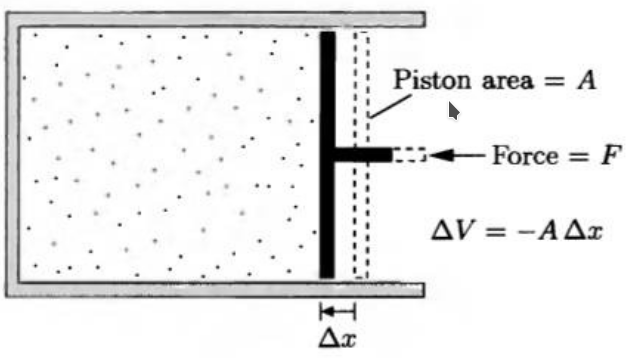
\includegraphics[width=0.5\textwidth]{Piston}
\end{center}
The only way we can exert a force on this gas system is by moving the piston
in what we'll define as the $x$ direction by some amount $\Delta x$. This
means that we can take the work equation we had before to be
\[ W = F\Delta x \]
Where a positive $\Delta x$ means the piston moves inward. We can write this
instead in terms of the volume and pressure, things that are more apparent
from the ideal gas law we've been working with:
\begin{align*}
	W_{on} &= P\Delta x\\
	       &= PA\Delta x\\
	       &= -P\Delta V
\end{align*}
Not ethat we made two mig assumptions here:
\begin{enumerate}
	\item \textbf{Quasistatic change}\\
		We assumed that as the piston moved, the gas was at equilibrium
		at every point in time. This is an idealization, but usually
		a good enough approximation.
	\item \textbf{Isobaric}\\
		We assumed that the pressure in the piston was constant.
		That is, we could pull the pressure out of an integral like
		so:
		\begin{align*}
			W &= -P\Delta V\\
			  &= -\int_{V_i}^{V_f} P(V)\d V\\
			  &= -P\int_{V_i}^{V_f} \d V
		\end{align*}
		For this isobaric assumption to be true, according to the ideal
		gas law, the temperature $T$ must be changing.
\end{enumerate}

Now, suppose we did some compression, but we kept the temperature constant
(ie. we did an \emph{isothermal} compression).
What must be the work done on the system now?
\begin{align*}
	W &= -\int_{V_i}^{V_f} P(V)\d V\\
	  &= -\int_{V_i}^{V_f}\frac{nRT}{V}\d V\\
	  &= -nRT\ln\left(\frac{V_f}{V_i}\right)
\end{align*}
We can no longer rely on a constant pressure, but we can rely on a constant
temperature and knowing the initial and final volumes. If we graph such an
isothermal compression on a Pressure-Volume plot, we can see what we
call an isotherm:

\begin{center}
\begin{tikzpicture}
\begin{axis}[
	axis lines = left,
	xlabel = {Volume},
	ylabel = {Pressure},
	xmin=0, xmax=1,
	ymin=0, ymax=1,
	xtick={0,0.25,0.75},
	xticklabels={,$V_f$,$V_i$},
	ytick={0},
	yticklabels={}
]

\addplot [
	domain=0.25:0.75,
	samples=100,
]
{0.2/(x)};

\addplot[only marks] coordinates {(0.25,0.8)(0.75,0.266667)};

	
\end{axis}
\end{tikzpicture}
\end{center}
For reasons we'll prove later, the total internal energy of a
monatomic ideal gas at any time is given by
\[ U = \frac{3}{2}N k_B T = \frac{3}{2} nRT \]
Note that the 3 in the numerator of that fraction comes from the number of
degrees of freedom for a single atom (all 3 translational degrees of freedom).
Note that the only non-constant term here is $T$. That means that if $T$
doesn't change, as in an isothermic compression or expansion, then the total
internal energy should be the same at the beginning as it is at the end, or
\[ \Delta U = 0 \]
We can use the first law of thermodynamics to conclude, then, that
\begin{align*}
	\Delta U &= 0\\
	Q + W &= 0\\
	Q &= -W
\end{align*}
This means that in order to maintain constant temperature during a compression,
heat must flow out of the system.

Lastly, we'll look at an adiabatic system: one where we compress or expand
our ideal gas in a chamber which is isolated from its environment (the most
important meaning of this: heat can't flow between the system and its
environment). If $Q$ can't flow at all, then that means we must have $Q=0$, so
\begin{align*}
	\Delta U &= \cancelto{0}{Q} + W\\
		 &= W
\end{align*}
We can use an infinitesimal change in energy for an ideal gas undergoing
adiabatic compression or expansion to show some interesting features:
\begin{align*}
	\d U = \frac32 N k_B \d T &= -P\d V\\
	\frac32 \cancel{N}\cancel{k_B}\d T &= -\frac{\cancel{N}\cancel{k_B}T}
		{V}\d V\\
	\frac32 \frac{\d T}{T} &= -\frac{\d V}{V}\\
	\frac32 \ln\left(\frac{T_f}{T_i}\right) &=
		-\ln\left(\frac{V_f}{V_i}\right)\\
	V_fT_f^{3/2} &= V_iT_i^{3/2}
\end{align*}
In other words, when an isolated system undergoes a change in volume (ie.
a compression or expansion), the quantity $VT^{3/2}$ is always constant.
By extension,
\begin{align*}
	VT^{3/2} &= \text{const.}\\
	V^{2/3}T &= \text{const.}'\\
	V^{2/3}\frac{PV}{nR} &= \text{const.}'\\
	V^{5/3}P &= \text{const.}''
\end{align*}
If we plot an isothermic compression (or expansion) along a Volume-Pressure
graph, we find that along an adiabat, $P\propto\frac{1}{V^{5/3}}$

\begin{center}
\begin{tikzpicture}
\begin{axis}[
	axis lines = left,
	xlabel = {Volume},
	ylabel = {Pressure},
	xmin=0, xmax=1,
	ymin=0, ymax=1,
	xtick={0,0.25,0.75},
	xticklabels={,$V_f$,$V_i$},
	ytick={0},
	yticklabels={}
]

\addplot [
	domain=0.25:0.75,
	samples=100,
]
{0.2/(x^(5/3))};

\addplot [
	domain=0.25:0.75,
	samples=100,
]
{0.2/(x)};
\addplot [
	domain=0.25:0.75,
	samples=100,
]
{0.2/(x-0.25)};

\end{axis}
\end{tikzpicture}
\end{center}


\subsubsection{Heat Capacities}
Heat capacity is defined as the amount of heat needed to raise the temperature
of an object per temperature degree increase (or the amount of heat needed to
raise the temperature of an object by 1$^\circ$C or 1K). Mathematically,
\[
	C \equiv \frac{Q}{\Delta T} = \frac{\Delta U - W}{\Delta T}
\]
Note that this is definitionally context-dependent: doing work on an object
changes its heat capacity. Practically, there aretwo types of heat capacity
that we talk about: heat capacity at constant volume, where no work is being
done on the system and threfore the volume of the container does not change,
and heat capacity at constant pressure, where the pressure in the container is
held constant (implying that the volume is changing).\\
Mathematically, we can write heat capacity at constant volume easily as a
differential, and solve it for the case of the monatomic ideal gas:
\begin{align*}
	C_V &= \left(\frac{\Delta U}{\Delta T}\right)_V
	= \left(\pder{U}{T}\right)_V\\
	&= \left.\frac{3}{2}N k_B \pder{T}{T}\right|_V\\
	&= \frac{3}{2}N k_B
\end{align*}
Similarly, at constant pressure, we can write the heat capacity using our
energy-work definitions:
\begin{align*}
	C_P &= \left.\frac{\Delta U - W}{\Delta T}\right|_P\\
	&= \left.\frac{\Delta U - (-P\Delta V)}{\Delta T}\right|_P\\
	&= \left(\pder{U}{T}\right)_P + P\left(\pder{V}{T}\right)_P\\
	&= \left.\frac{3}{2}N k_B \pder{T}{T}\right|_P +
		\left.P\left(\frac{N k_B}{P}\right)\pder{T}{T}\right|_P\\
	&= \frac{5}{2}N k_B
\end{align*}
We can see that $C_P > C_V$ by a difference of $N k_B$ (or, more
mathematically, $C_P - C_V = N k_B$). Here's an intuitive reason why: If the
volume can't expand and we put in energy, it takes much less energy to increase
the heat than it would if some of that energy had to go towards the work of
expansion or contraction.\\
For non-monatomic ideal gases, we can extend these. In general, we can write
the internal energy of a system as a function of the degrees of freedom $f$:
\[
	U = \frac{f}{2} N k_B T = \frac{f}{2} nRT
\]
In the case of a monatomic ideal gas, where there are 3 (translational) degrees
of freedom, we have the internal energy equation that we've seen already. In a
case like $H_2$, we have 3 translational degrees of freedom, 2 vibrational
degrees of freedom (kinetic and potential energy stored in bond vibrations),
and 2 rotational degrees of freedom (note that axis rotation isn't included
because in quantum mechanics, these particles aren't distinguishable and we
can't keep track of axis rotation, so no energy can be stored there). In this
case,
\[
	U = \frac{7}{2} N k_B T = \frac{7}{2}nRT
\]
We can see the effects of this on $C_V$ in the graph below:
\begin{center}
	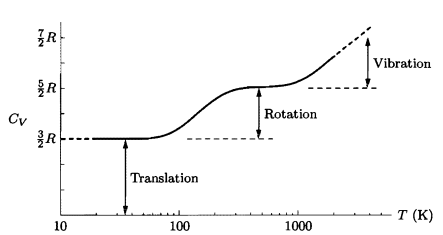
\includegraphics[width=0.75\textwidth]{HC_V.png}
\end{center}

\subsubsection{Phase Transitions and Latent Heat}
At phase transitions, we can heat without necessarily increasing temperature.
This means two things. First, we can find that $C_V \to \infty$ as the
temperature approaches the critical temperature (ie. the temperature at which
the phase transition occurs). Second, this means that we need to introduce a
new quantity that specifies the amount of heat required to increase the
temperature and change the phase of a material with mass $m$.
We call this the latent heat, $L$, where
\[
	L = \frac{Q}{m}
\]

\subsubsection{Enthalpy}
We run into constant-pressure processes a lot. In constant-pressure processes,
it can be time-consuming to keep track of the work done after a while, but we
can introduce something to make that easier: rather than talking about the
energy of a system, we can find it convenient to talk about the enthalpy. The
enthalpy is defined as
\[
	H \equiv U + PV
\]
At constant pressure, the enthalpy is just the heat flowing into the system:
\begin{align*}
	\Delta H &= \Delta U + P \Delta V\\
	&= Q - P\Delta V + P\Delta V\\
	&= Q
\end{align*}
And thus,
\[
	C_P = \left.\pder{Q}{T}\right|_P = \left.\pder{H}{T}\right|_P
\]

\subsection{The Second Law, Engines, and Refrigerators}
% Syllabus: Carnot Engine, Second Law, Entropies of mixing (4.1-4.2, 2.1, 2.4-2.6)
\subsubsection{The Carnot Engine}
A heat engine is a device which absorbs heat and converts that energy into
work. But not all absorbed heat can be converted into work (this is one way of
stating the second law of thermodynamics). We'll explain why a little later
when we introduce entropy. Here's a brief energy-flow diagram of what a heat
enegine looks like: energy flows from the hot reservoir to generate work, with
the leftover heat flowing into the cold reservoir:
\begin{center}
	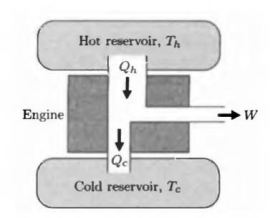
\includegraphics[width=0.5\textwidth]{Heat_Engine.png}
\end{center}
We define the efficiency, $\epsilon$, of a system as the ratio of useful work,
to heat absorbed:
\[
	\epsilon = \frac{W}{Q_H} = \frac{Q_H^{the.} - Q_C^{the.}}{Q_H^{the.}}
	\leq \frac{Q_H^{act.} - Q_C^{act.}}{Q_H^{act.}}
\]
We can draw the cycle of an engine on a graph of pressure vs. pressure, where
the work done would be given by the area between the curves describing the
pressure as a function of volume. We can deform the path on the diagram to be
in terms of adiabats and isotherms, while keeping the area (work) constant.
\begin{center}
	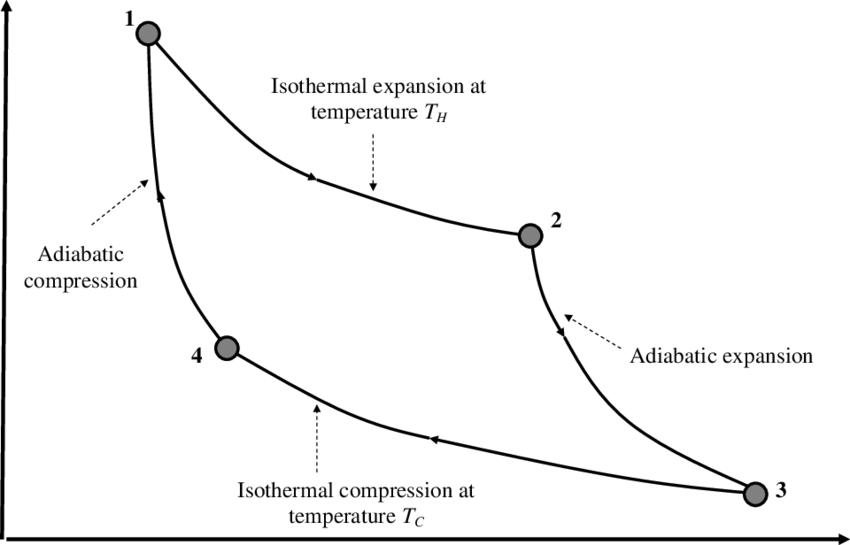
\includegraphics[width=0.5\textwidth]{Carnot.png}
\end{center}
We call the cycle thus described the Carnot cycle. Here's a description:\\
\begin{align*}
1\to 2&: \text{Isotherm}\\
	&& U &= Q_h + W = 0&\\
	&& W &= -Q_h\\
	&& Q_h &= T_h(S_2-S_1)\\
2\to3&: \text{Adiabatic expansion}\\
	&& \Delta U &= \frac{3}{2}Nk_B(T_c-T_h)\\
	&& &= W\\
3\to4&: \text{Isothermal compression}\\
	&& Q &= T_C(S_4-S_3)\\
	&& &= T_C(S_1-S_2)\\
	&& &= -Q_C\\
4\to1&: \text{Adiabatic compression}\\
	&& \Delta U &= \frac{3}{2}Nk_B(T_h-T_c)
\end{align*}
We defined a state variable $S$ here---there must be some internal variable
that defines the difference of state between 1 and 2. We call this entropy.\\
Using the relations we see in that cycle, we can re-write the efficiency of an
engine as
\begin{align*}
	\epsilon &= \frac{Q_h - Q_c}{Q_h}\\
	&= \frac{T_h - T_c}{T_h}\\
	&= 1 - \frac{T_c}{T_h}
\end{align*}
We can see here clearly that even in the limit where we consider only
theoretical $Q_h$ and $Q_c$, the efficiency must be less than 1. We can also
say that
\[
	Q_h^{act.} \leq T\Delta S = Q_h^{theo.}
\]

\paragraph{Regrigerators}
We can reverse this cycle/process and get what we call a refrigerator. In this
case, we say that we take heat out of the cold reservoir and put it in the hot
reservoir, but in order to do so, we must use some work. Rather than talking
about the efficiency of a refrigerator, we usually talk about the coefficient
of performance:
\[
	\text{COP} &= \frac{Q_c}{W}\\
	&= \frac{T_c}{T_h-T_c}
\]

\subsubsection{Two-State and Multi-State Systems}
We'll need to take a brief statistical interlude. Suppose we flip a coin 3
times. If we get two heads and one tails, we call this a macrostate. There are
3 possible ways to get this macrostate: HHT, HTH, and THH. These three ways are
called microstates. In a full sentence, we might say that there are 3
microstates consistent with our macrostate. Alternatively, we might say that
the multiplicity, $\Omega$, of the macrostate is 3. We can find the
multiplicity generally by taking the binomial coefficient. To find the
multiplicity of a macrostate with $N$ number of events (ie. flips) and $n$ of a
certain outcome (ie. heads), we would do:
\[
	\Omega = \begin{pmatrix}N\\n\end{pmatrix} = \frac{N!}{n!(N-n)!}
\]
If there are more than 2 possible outcomes (or, really, we could do this with 2
possible outcomes), we write this as
\[
	\Omega = \begin{pmatrix}N\\n_1\cdots n_i\end{pmatrix}
	= \frac{N!}{n_1!\cdots n_i!}
\]
As long as the sum of the small $n$ comes out to $N$.

\subsubsection{The Second Law of Thermodynamics}
\subsubsection{Large Systems}
\subsubsection{The Ideal Gas}
\subsubsection{Entropy}

\subsection{Interactions and Implications}
% Syllabus: Temperature, equilibrium and potentials (3.1-3.2, 3.4-3.6)
\subsubsection{Temperature}
\subsubsection{Entropy and Heat}
\subsubsection{Mechanical Equilibrium and Pressure}
\subsubsection{Diffusive Equilibrium and Chemical Potential}

\subsection{Free Energy and Chemical Thermodynamics}
% Syllabus: Enthalpy, Helmholtz free energy, Gibbs free energy, Maxwell and cyclic relations (5.1-5.2)
\subsubsection{Free Energy as Available Work}
\subsubsection{Free Energy as a Force Toward Equilibrium}
% Syllabus: Phase transformations (5.3)
\subsubsection{Phase Transofrmations of Pure Substances}

\section{Statistics}

% Syllabus: Probabilities, manipulating probabilities, CDFs, fundamental theorem of simulation, moments, central limit theorem
% Syllabus: Likelihoods, Bayes' theorem, manipulating probabilities, posteriors and parameter estimation
% Syllabus: Maximum entropy, density estimation, manipulating distributions and sampling problems

\section{Statistical Mechanics}

\subsection{Boltzmann Statistics}
% Syllabus: Bolzmann statistics and partition functions for discrete systems
\subsubsection{The Boltzmann Factor}
\subsubsection{Average Values}
% Syllabus: Boltzmann weights and partition functions for continuous systems
\subsubsection{Partition Functions and Free Energy}
% Syllabus: Classical statistical mechanics + Monte Carlo, Metropolis-Hastings
\subsubsection{Partition Functions for Composite Systems}
\subsubsection{Ideal Gas Revisited}
\subsubsection{Monte Carlo, Metropolis-Hastings}

\subsection{Quantum Statistics}
% Syllabus: Quantum statistics, bosons and fermions
\subsubsection{The Gibbs Factor}
\subsubsection{Bosons and Fermions}
% Syllabus: Applications of Quantum Statistis
\subsubsection{Degenerate Fermi Gases}
\subsubsection{Blackbody Radiation}
\subsubsection{Debye Theory of Solids}

\end{document}
